\section*{Analysis}
\label{sec:analysis}

The emulator is used to perform the debugging (although it does not seem to be able to run RenderScript code).
To run the code, we are using two devices for the analysis.
The first is a Nexus 7 with the following specs:

\begin{verbatim}
    CPU: Qualcomm Snapdragon S4 Pro, 1.5GHz
    GPU: Adreno 320, 400MHz
    Memory - 2 GB
    Storage 32 GB
\end{verbatim}

The second is a Samsung Galaxy Nexus with the following specs:

\begin{verbatim}
    CPU: ARMv7, 2 cores, 1200 Mhz, SIMD NEON
    Memory: 694, JVM max: 96 MB
    GPU: PowerVR SGX 540.
\end{verbatim}


\subsection*{Perliminary Results}

While we do have implementations for 3 out of the 4 benchmarks we promised in the proposal schedule,
  our results only show part of those.
This is primarily due to a lack of time configuring the devices to run the benchmarks.


\begin{figure}[t!]
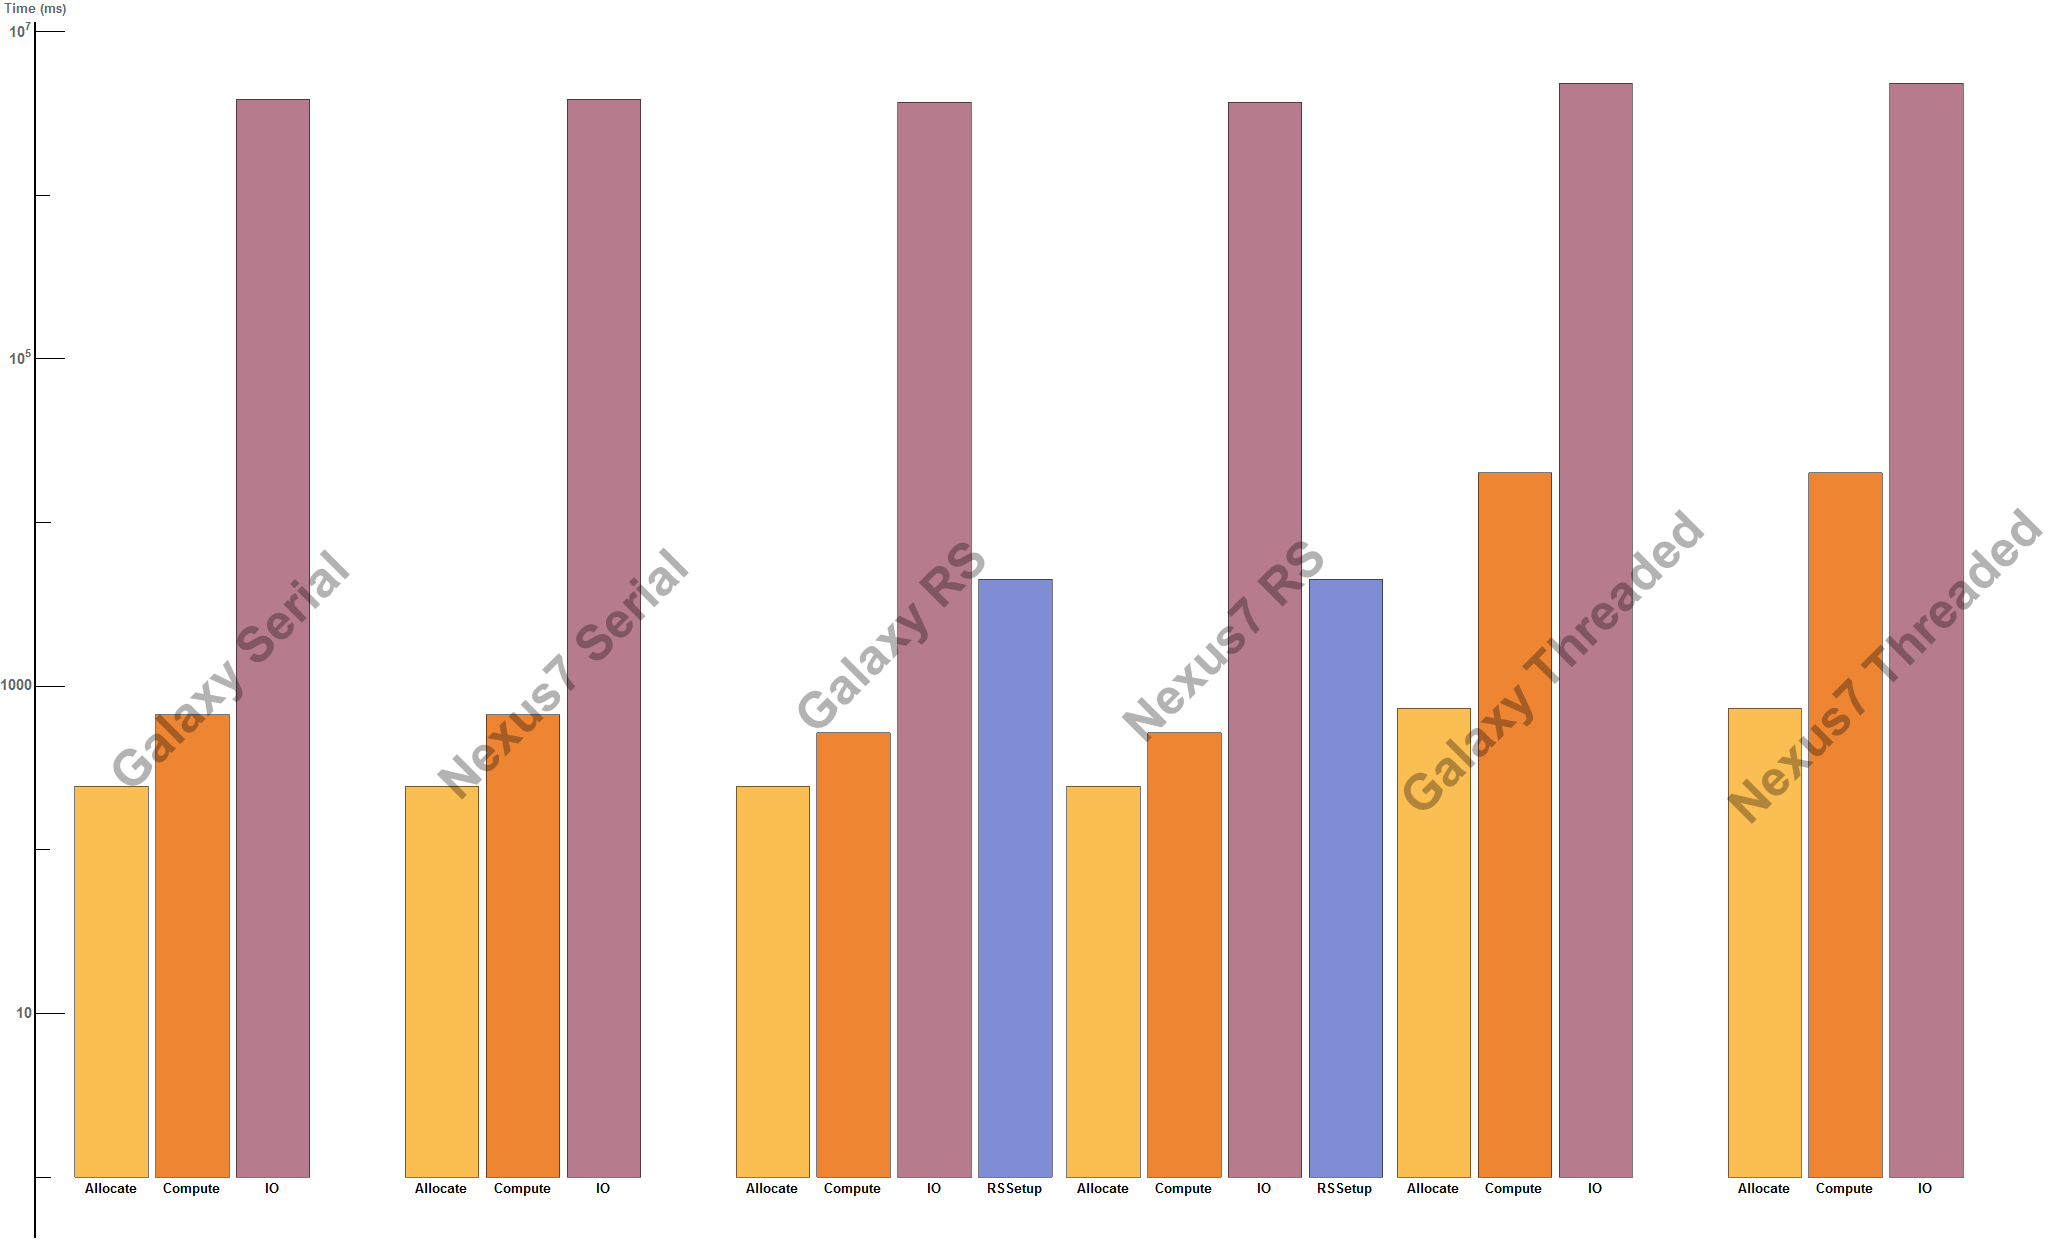
\includegraphics[scale=0.125]{VectorAdd.png}
\caption{VectorAdd Benchmark.}
\label{fig:schedule}
\centering
\end{figure}



\begin{figure}[t!]
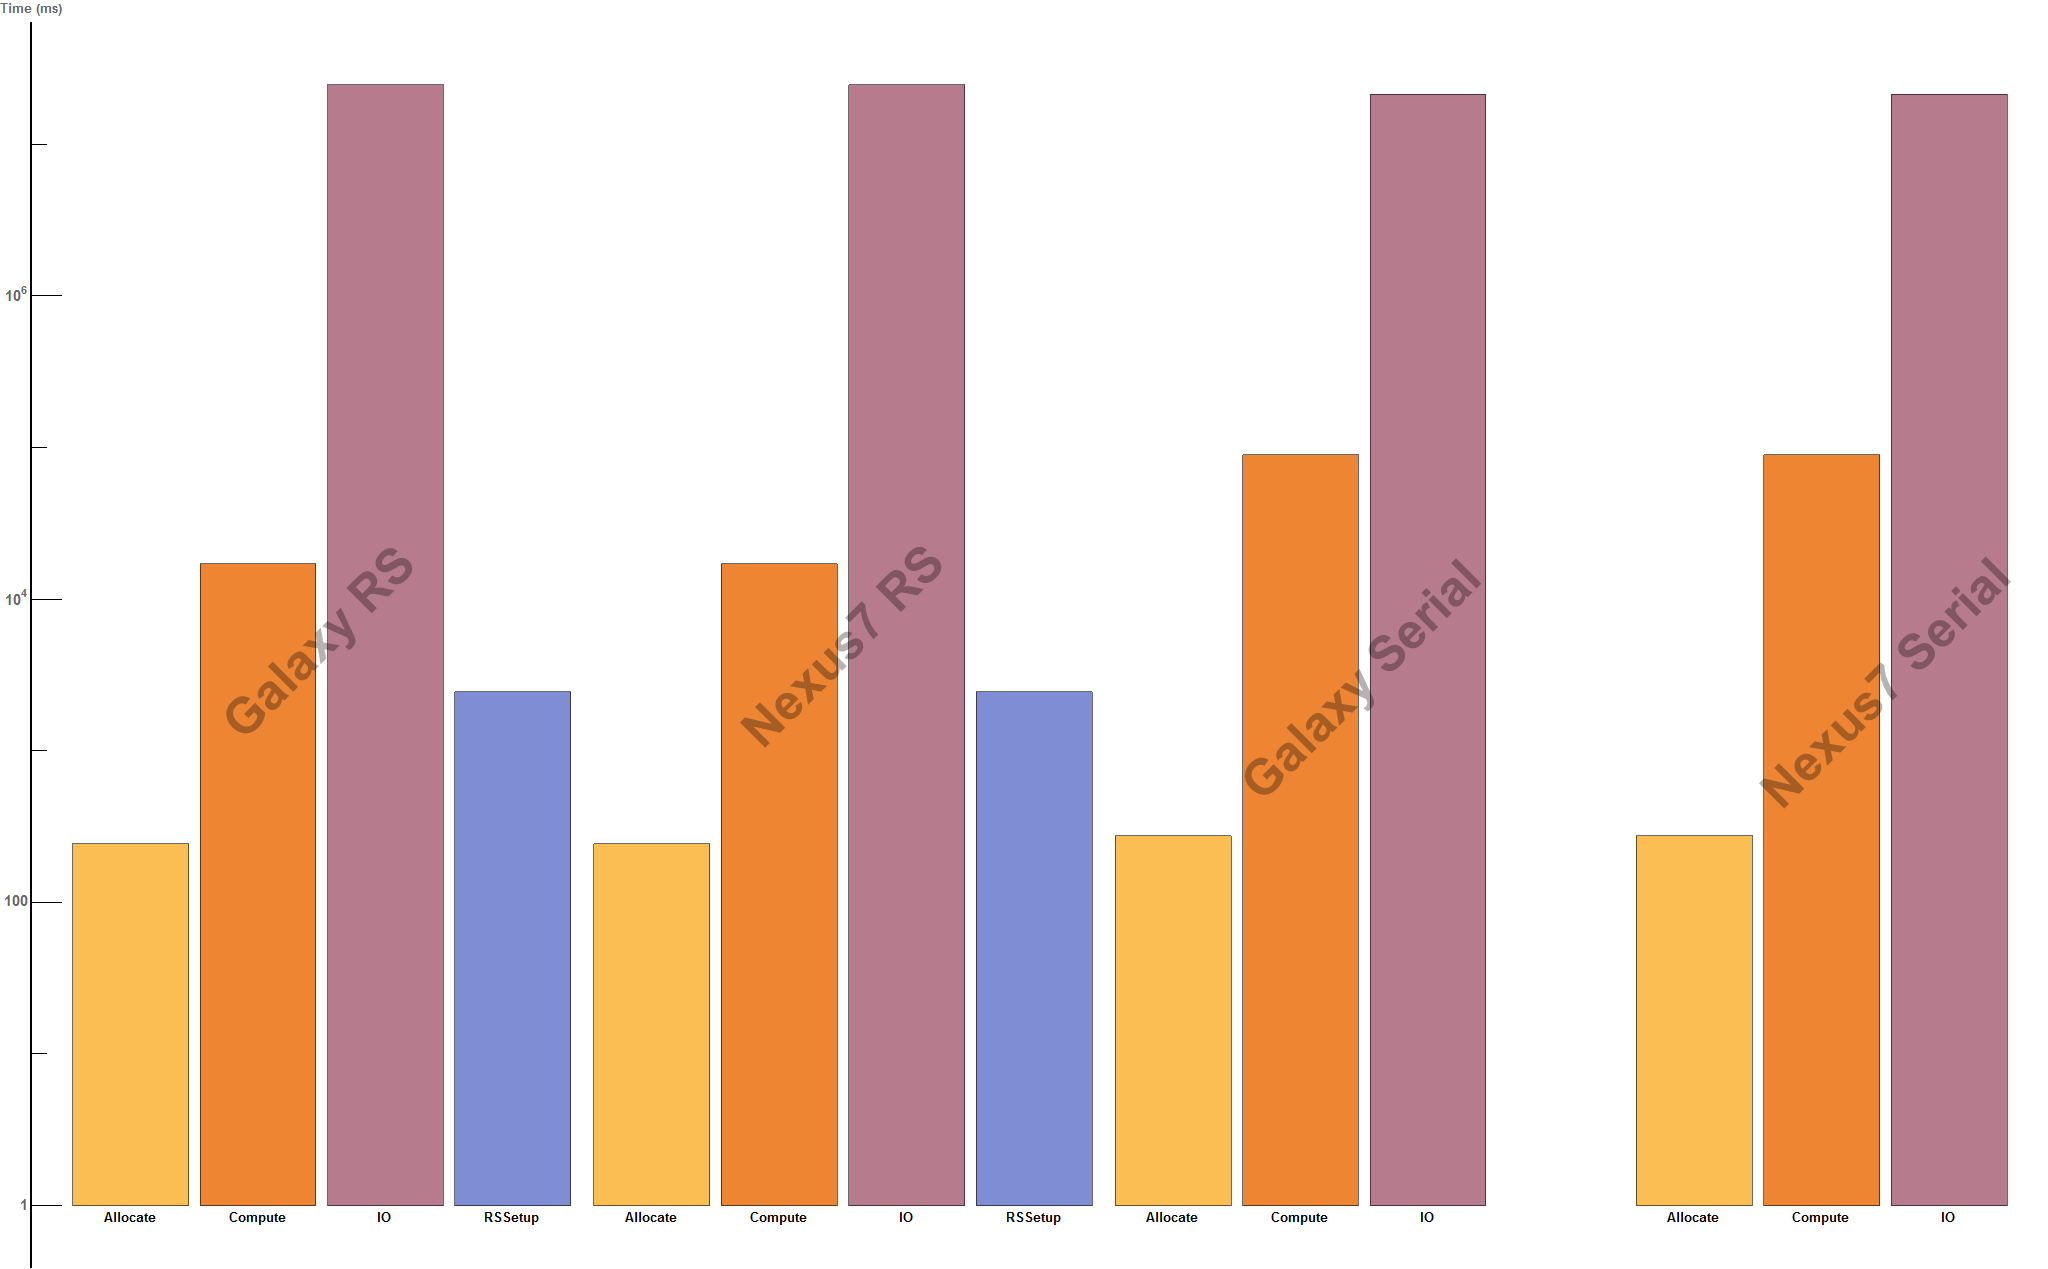
\includegraphics[scale=0.125]{Sgemm.png}
\caption{Matrix Matrix Multiplication Benchmark.}
\label{fig:schedule}
\centering
\end{figure}



\begin{figure}[t!]
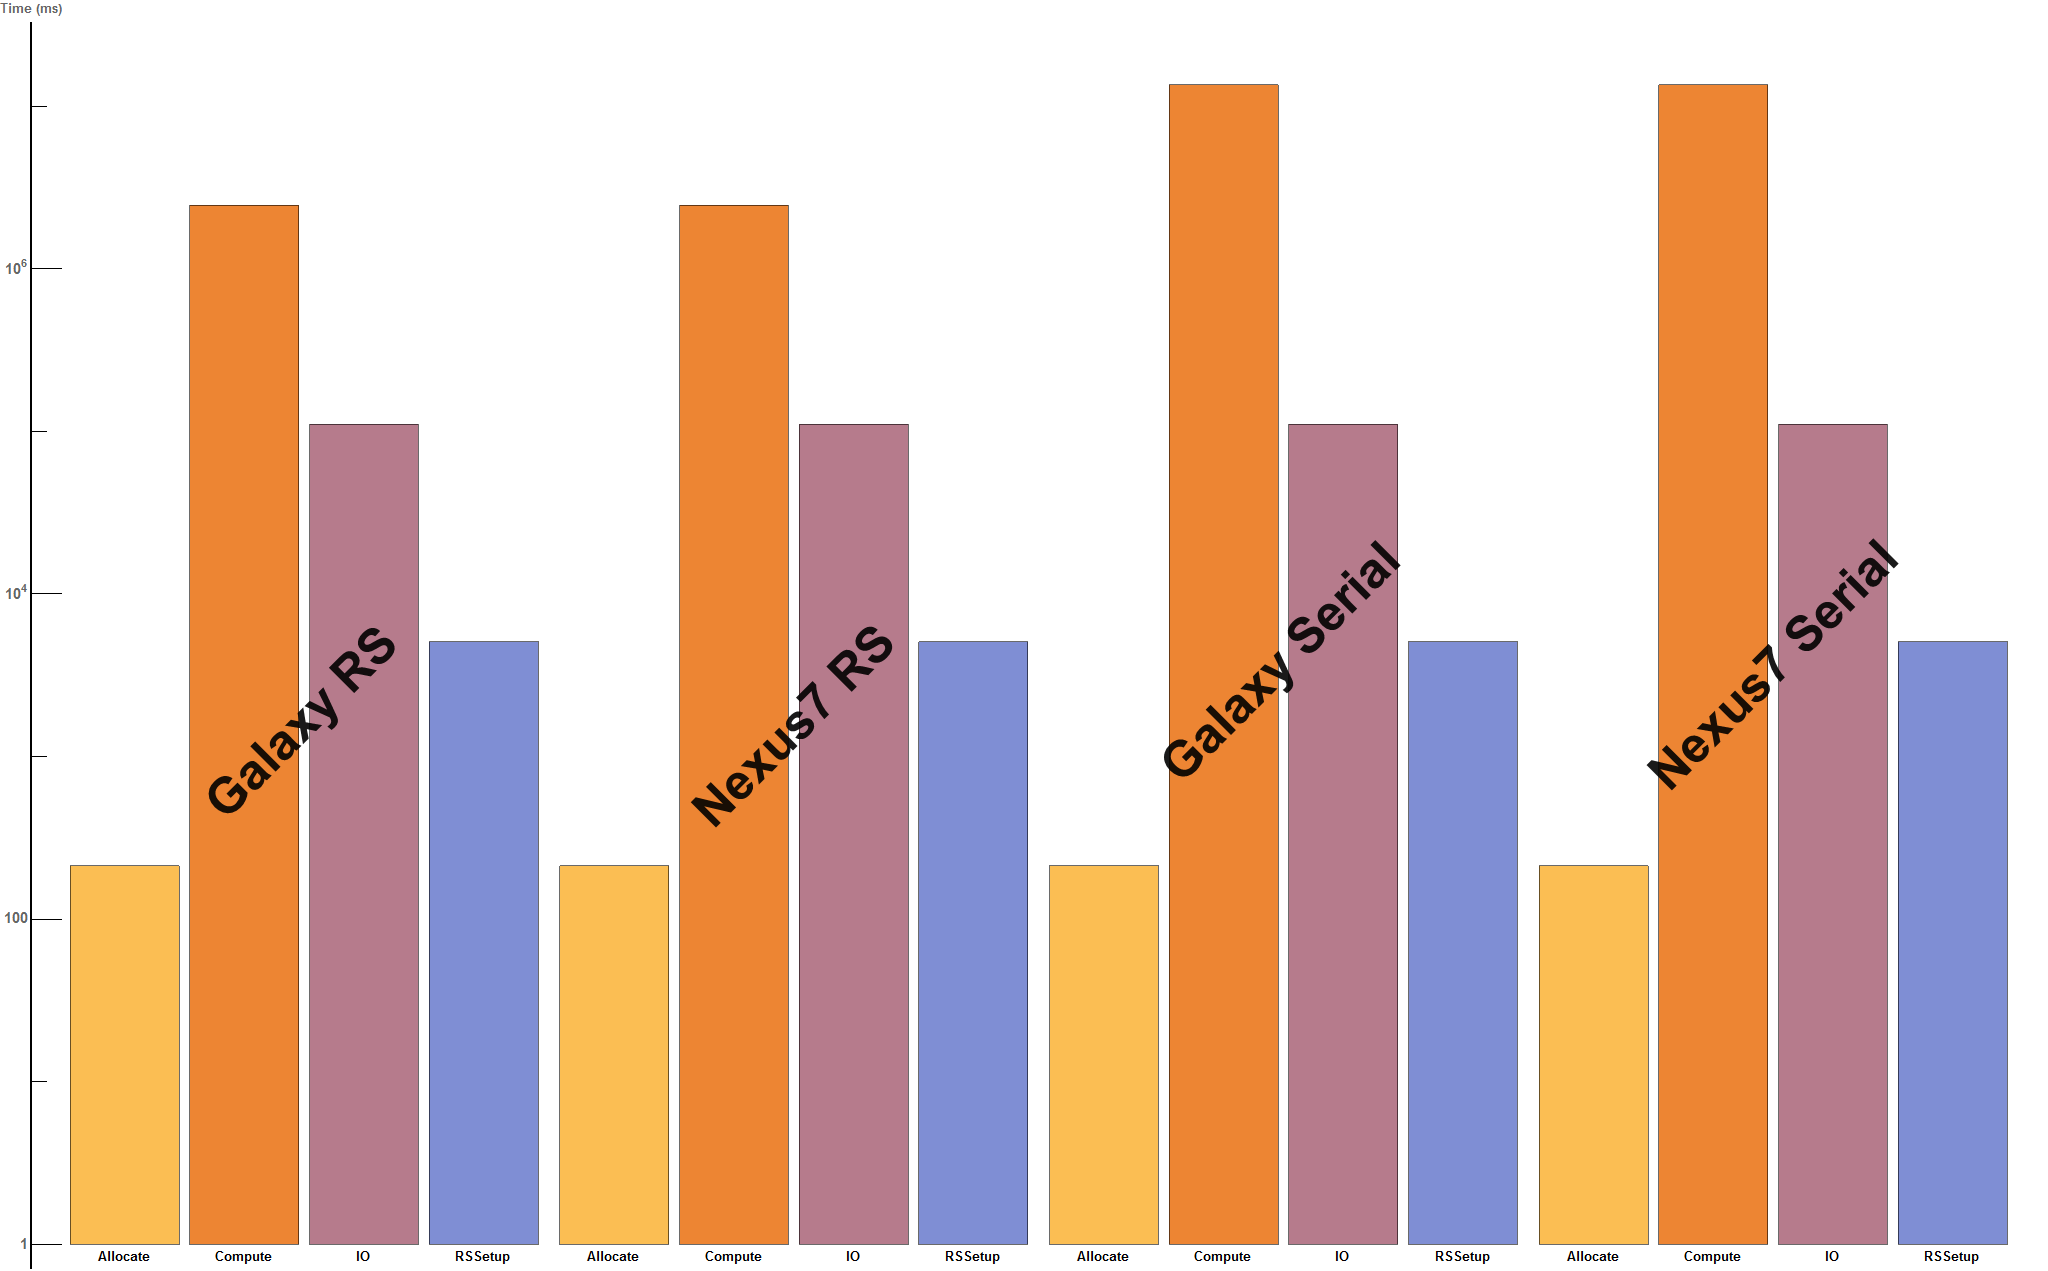
\includegraphics[scale=0.125]{Stencil.png}
\caption{Stencil Benchmark.}
\label{fig:schedule}
\centering
\end{figure}


While these graphs have the infromation, they are not presented in the clearest way.
Future work would merge the datasets not just by devices, but also by different benchmark implementations.

